% Options for packages loaded elsewhere
\PassOptionsToPackage{unicode}{hyperref}
\PassOptionsToPackage{hyphens}{url}
\PassOptionsToPackage{dvipsnames,svgnames,x11names}{xcolor}
%
\documentclass[
  letterpaper,
  DIV=11,
  numbers=noendperiod]{scrartcl}

\usepackage{amsmath,amssymb}
\usepackage{iftex}
\ifPDFTeX
  \usepackage[T1]{fontenc}
  \usepackage[utf8]{inputenc}
  \usepackage{textcomp} % provide euro and other symbols
\else % if luatex or xetex
  \usepackage{unicode-math}
  \defaultfontfeatures{Scale=MatchLowercase}
  \defaultfontfeatures[\rmfamily]{Ligatures=TeX,Scale=1}
\fi
\usepackage{lmodern}
\ifPDFTeX\else  
    % xetex/luatex font selection
\fi
% Use upquote if available, for straight quotes in verbatim environments
\IfFileExists{upquote.sty}{\usepackage{upquote}}{}
\IfFileExists{microtype.sty}{% use microtype if available
  \usepackage[]{microtype}
  \UseMicrotypeSet[protrusion]{basicmath} % disable protrusion for tt fonts
}{}
\makeatletter
\@ifundefined{KOMAClassName}{% if non-KOMA class
  \IfFileExists{parskip.sty}{%
    \usepackage{parskip}
  }{% else
    \setlength{\parindent}{0pt}
    \setlength{\parskip}{6pt plus 2pt minus 1pt}}
}{% if KOMA class
  \KOMAoptions{parskip=half}}
\makeatother
\usepackage{xcolor}
\usepackage[left=1in,right=1in,top=1in,bottom=1in]{geometry}
\setlength{\emergencystretch}{3em} % prevent overfull lines
\setcounter{secnumdepth}{-\maxdimen} % remove section numbering
% Make \paragraph and \subparagraph free-standing
\ifx\paragraph\undefined\else
  \let\oldparagraph\paragraph
  \renewcommand{\paragraph}[1]{\oldparagraph{#1}\mbox{}}
\fi
\ifx\subparagraph\undefined\else
  \let\oldsubparagraph\subparagraph
  \renewcommand{\subparagraph}[1]{\oldsubparagraph{#1}\mbox{}}
\fi

\usepackage{color}
\usepackage{fancyvrb}
\newcommand{\VerbBar}{|}
\newcommand{\VERB}{\Verb[commandchars=\\\{\}]}
\DefineVerbatimEnvironment{Highlighting}{Verbatim}{commandchars=\\\{\}}
% Add ',fontsize=\small' for more characters per line
\usepackage{framed}
\definecolor{shadecolor}{RGB}{241,243,245}
\newenvironment{Shaded}{\begin{snugshade}}{\end{snugshade}}
\newcommand{\AlertTok}[1]{\textcolor[rgb]{0.68,0.00,0.00}{#1}}
\newcommand{\AnnotationTok}[1]{\textcolor[rgb]{0.37,0.37,0.37}{#1}}
\newcommand{\AttributeTok}[1]{\textcolor[rgb]{0.40,0.45,0.13}{#1}}
\newcommand{\BaseNTok}[1]{\textcolor[rgb]{0.68,0.00,0.00}{#1}}
\newcommand{\BuiltInTok}[1]{\textcolor[rgb]{0.00,0.23,0.31}{#1}}
\newcommand{\CharTok}[1]{\textcolor[rgb]{0.13,0.47,0.30}{#1}}
\newcommand{\CommentTok}[1]{\textcolor[rgb]{0.37,0.37,0.37}{#1}}
\newcommand{\CommentVarTok}[1]{\textcolor[rgb]{0.37,0.37,0.37}{\textit{#1}}}
\newcommand{\ConstantTok}[1]{\textcolor[rgb]{0.56,0.35,0.01}{#1}}
\newcommand{\ControlFlowTok}[1]{\textcolor[rgb]{0.00,0.23,0.31}{#1}}
\newcommand{\DataTypeTok}[1]{\textcolor[rgb]{0.68,0.00,0.00}{#1}}
\newcommand{\DecValTok}[1]{\textcolor[rgb]{0.68,0.00,0.00}{#1}}
\newcommand{\DocumentationTok}[1]{\textcolor[rgb]{0.37,0.37,0.37}{\textit{#1}}}
\newcommand{\ErrorTok}[1]{\textcolor[rgb]{0.68,0.00,0.00}{#1}}
\newcommand{\ExtensionTok}[1]{\textcolor[rgb]{0.00,0.23,0.31}{#1}}
\newcommand{\FloatTok}[1]{\textcolor[rgb]{0.68,0.00,0.00}{#1}}
\newcommand{\FunctionTok}[1]{\textcolor[rgb]{0.28,0.35,0.67}{#1}}
\newcommand{\ImportTok}[1]{\textcolor[rgb]{0.00,0.46,0.62}{#1}}
\newcommand{\InformationTok}[1]{\textcolor[rgb]{0.37,0.37,0.37}{#1}}
\newcommand{\KeywordTok}[1]{\textcolor[rgb]{0.00,0.23,0.31}{#1}}
\newcommand{\NormalTok}[1]{\textcolor[rgb]{0.00,0.23,0.31}{#1}}
\newcommand{\OperatorTok}[1]{\textcolor[rgb]{0.37,0.37,0.37}{#1}}
\newcommand{\OtherTok}[1]{\textcolor[rgb]{0.00,0.23,0.31}{#1}}
\newcommand{\PreprocessorTok}[1]{\textcolor[rgb]{0.68,0.00,0.00}{#1}}
\newcommand{\RegionMarkerTok}[1]{\textcolor[rgb]{0.00,0.23,0.31}{#1}}
\newcommand{\SpecialCharTok}[1]{\textcolor[rgb]{0.37,0.37,0.37}{#1}}
\newcommand{\SpecialStringTok}[1]{\textcolor[rgb]{0.13,0.47,0.30}{#1}}
\newcommand{\StringTok}[1]{\textcolor[rgb]{0.13,0.47,0.30}{#1}}
\newcommand{\VariableTok}[1]{\textcolor[rgb]{0.07,0.07,0.07}{#1}}
\newcommand{\VerbatimStringTok}[1]{\textcolor[rgb]{0.13,0.47,0.30}{#1}}
\newcommand{\WarningTok}[1]{\textcolor[rgb]{0.37,0.37,0.37}{\textit{#1}}}

\providecommand{\tightlist}{%
  \setlength{\itemsep}{0pt}\setlength{\parskip}{0pt}}\usepackage{longtable,booktabs,array}
\usepackage{calc} % for calculating minipage widths
% Correct order of tables after \paragraph or \subparagraph
\usepackage{etoolbox}
\makeatletter
\patchcmd\longtable{\par}{\if@noskipsec\mbox{}\fi\par}{}{}
\makeatother
% Allow footnotes in longtable head/foot
\IfFileExists{footnotehyper.sty}{\usepackage{footnotehyper}}{\usepackage{footnote}}
\makesavenoteenv{longtable}
\usepackage{graphicx}
\makeatletter
\def\maxwidth{\ifdim\Gin@nat@width>\linewidth\linewidth\else\Gin@nat@width\fi}
\def\maxheight{\ifdim\Gin@nat@height>\textheight\textheight\else\Gin@nat@height\fi}
\makeatother
% Scale images if necessary, so that they will not overflow the page
% margins by default, and it is still possible to overwrite the defaults
% using explicit options in \includegraphics[width, height, ...]{}
\setkeys{Gin}{width=\maxwidth,height=\maxheight,keepaspectratio}
% Set default figure placement to htbp
\makeatletter
\def\fps@figure{htbp}
\makeatother

\usepackage{booktabs}
\usepackage{longtable}
\usepackage{array}
\usepackage{multirow}
\usepackage{wrapfig}
\usepackage{float}
\usepackage{colortbl}
\usepackage{pdflscape}
\usepackage{tabu}
\usepackage{threeparttable}
\usepackage{threeparttablex}
\usepackage[normalem]{ulem}
\usepackage{makecell}
\usepackage{xcolor}
\usepackage{fvextra}
\DefineVerbatimEnvironment{Highlighting}{Verbatim}{breaklines,commandchars=\\\{\}}
\DefineVerbatimEnvironment{OutputCode}{Verbatim}{breaklines,commandchars=\\\{\}}
\KOMAoption{captions}{tableheading}
\makeatletter
\@ifpackageloaded{caption}{}{\usepackage{caption}}
\AtBeginDocument{%
\ifdefined\contentsname
  \renewcommand*\contentsname{Table of contents}
\else
  \newcommand\contentsname{Table of contents}
\fi
\ifdefined\listfigurename
  \renewcommand*\listfigurename{List of Figures}
\else
  \newcommand\listfigurename{List of Figures}
\fi
\ifdefined\listtablename
  \renewcommand*\listtablename{List of Tables}
\else
  \newcommand\listtablename{List of Tables}
\fi
\ifdefined\figurename
  \renewcommand*\figurename{Figure}
\else
  \newcommand\figurename{Figure}
\fi
\ifdefined\tablename
  \renewcommand*\tablename{Table}
\else
  \newcommand\tablename{Table}
\fi
}
\@ifpackageloaded{float}{}{\usepackage{float}}
\floatstyle{ruled}
\@ifundefined{c@chapter}{\newfloat{codelisting}{h}{lop}}{\newfloat{codelisting}{h}{lop}[chapter]}
\floatname{codelisting}{Listing}
\newcommand*\listoflistings{\listof{codelisting}{List of Listings}}
\makeatother
\makeatletter
\makeatother
\makeatletter
\@ifpackageloaded{caption}{}{\usepackage{caption}}
\@ifpackageloaded{subcaption}{}{\usepackage{subcaption}}
\makeatother
\ifLuaTeX
  \usepackage{selnolig}  % disable illegal ligatures
\fi
\usepackage{bookmark}

\IfFileExists{xurl.sty}{\usepackage{xurl}}{} % add URL line breaks if available
\urlstyle{same} % disable monospaced font for URLs
\hypersetup{
  pdftitle={Butterfly Ballot Blunder: An Investigation of the 2000 Presidential Election},
  pdfauthor={Dani Justo and Zoe Khan},
  colorlinks=true,
  linkcolor={blue},
  filecolor={Maroon},
  citecolor={Blue},
  urlcolor={Blue},
  pdfcreator={LaTeX via pandoc}}

\title{Butterfly Ballot Blunder: An Investigation of the 2000
Presidential Election}
\author{Dani Justo and Zoe Khan}
\date{2025-03-05}

\begin{document}
\maketitle

\section{Introduction}\label{introduction}

The 2000 U.S. presidential race was a highly contested election between
Al Gore and George W. Bush, with the latter eventually winning by a hair
due to Florida voters. However, something strange was afoot: people
noticed that the ``butterfly'' ballot design for Palm Beach county in
Florida was associated with a very high vote percentage for another
candidate, Pat Buchanan. It was theorized that the ballot design led
people to inadvertently vote for Buchanan instead of Gore. Our goal in
this report is to analyze the relationship between votes for Bush and
Buchanan in order to predict how many votes were potentially miscast.

\section{Data Description}\label{data-description}

\subsection{Ask about what summary statistics should be
included!!!}\label{ask-about-what-summary-statistics-should-be-included}

For our data analysis, we used the The ``Dramatic U.S. Presidential
Election of 2000'' data set from the \texttt{Sleuth2} package. This data
set includes the number of votes for Buchanan and Bush in all 67
counties in Florida during the 2000 U.S. presidential election. We want
to see if the confusing ``butterfly'' layout of the ballot used in Palm
Beach county caused the discrepancy in votes between Bush and Buchanan,
so we've removed Palm Beach county from our data set. This allows us to
observe relationship between Bush and Buchanan's votes under ``normal''
circumstances, namely, if the election really hadn't been affected by
the ballot.

The summary statistics in the table below suggest that Bush received
more votes than Buchanan in Florida on average.

\begin{table}[H]
\centering
\begin{tabular}[t]{cc}
\toprule
Mean Bush & Mean Buchanan\\
\midrule
41696.82 & 210.76\\
\bottomrule
\end{tabular}
\end{table}

The scatter plot displayed below has a correlation coefficient of 0.867,
suggesting a strong positive association between the number of votes for
Bush and the number of votes for Buchanan. The \(R^2\) of the linear
regression model is 0.862 indicates that the number of votes for Bush
account for 86.2\% of the variability in the number of votes for
Buchanan.

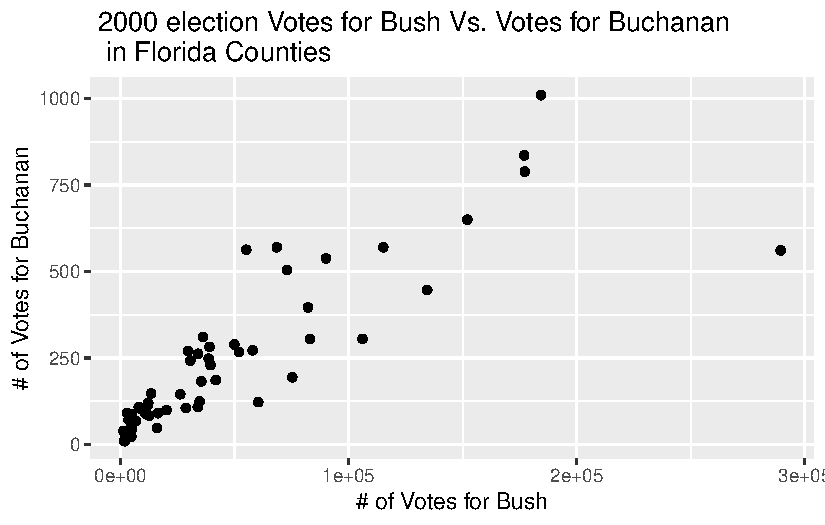
\includegraphics{case-study-template_files/figure-pdf/unnamed-chunk-4-1.pdf}

\section{Modeling Process}\label{modeling-process}

When we explored an initial linear model, we found violations of
linearity, equal variance, and normality, so we decided to use a
transformed model to rectify this issue. After some experimentation, we
found that a double-log transformation satisfied conditions and would
allow us to continue with our inquiry. Let \(Bush_i\) denote the votes
for Bush, and \(Buchanan_i\) denote the votes for Buchanan. Our final
transformed linear model is
\[E[log(Buchanan_i)|log(Bush_i)] = \beta_0 + \beta_1log(Bush_i)\]

The null hypothesis is that there is no relationship between votes for
Bush and Buchanan. The alternative hypothesis is there there is a
relationship: \[H_0 = \beta_1 = 0\] \[H_A = \beta_1 \neq 0\] The
estimates and standard errors of the model parameters are below:

\begin{table}[H]
\centering
\begin{tabular}[t]{lcccc}
\toprule
  & Estimate & Std. Error & t value & P-value\\
\midrule
(Intercept) & -2.34 & 0.35 & -6.61 & 0\\
log(Bush2000) & 0.73 & 0.04 & 20.32 & 0\\
\bottomrule
\end{tabular}
\end{table}

We get a very small p-value (\(\alpha\) = 0.05), so we reject the null
hypothesis and conclude that there is a relationship between votes for
Bush and Buchanan. In our prediction interval, we are 95\% confident
that an individual county with 152,846 votes for Bush would have between
250 and 1,394 votes for Buchanan. However, the true number of votes for
Buchanan was 3,407, which is well out of range of the prediction
interval. Taking the difference between the true estimate and the
interval values, we might predict that between 1,763 and 3,157 votes
were miscast.

\section{Conclusions}\label{conclusions}

From our analysis, we conclude that the number of votes for Buchanan in
Palm Beach county was indeed discrepant, falling outside the range of
values we might expect in an election where the butterfly ballot had not
been used.

Our analysis is limited to the relationship between the number of votes
for Bush and Buchanan, but does not account for how votes for may have
been miscast for other candidates as a result of the butterfly ballot.
Additionally, although we estimated that between 1,763 and 3,157 were
miscast in favor Buchanan, our estimation is limited by a lack of
information concerning the number of votes we could expect were intended
for Buchanan, potentially allowing us to overestimate or underestimate
the expected range of values for the number of miscast votes.

Because our study is observational, we can derive no causal effect.

There is a slight left skew in the distribution of the residuals in the
normality plot, but it is slight so we were not concerned that this
severely violates the normality condition.

\section{R Appendix}\label{r-appendix}

\begin{Shaded}
\begin{Highlighting}[]
\CommentTok{\# Import packages}
\FunctionTok{library}\NormalTok{(tidyverse)}
\FunctionTok{library}\NormalTok{(Sleuth2)      }
\FunctionTok{library}\NormalTok{(kableExtra) }
\FunctionTok{library}\NormalTok{(performance)}
\FunctionTok{library}\NormalTok{(broom)}
\FunctionTok{library}\NormalTok{(equatiomatic)}

\CommentTok{\# Loading the case study data}
\NormalTok{election }\OtherTok{\textless{}{-}}\NormalTok{ Sleuth2}\SpecialCharTok{::}\NormalTok{ex0825}

\CommentTok{\# Creating a second data set with Palm Beach County excluded}
\NormalTok{election\_wo\_pb }\OtherTok{\textless{}{-}}\NormalTok{ election }\SpecialCharTok{|\textgreater{}} \FunctionTok{filter}\NormalTok{(County }\SpecialCharTok{!=} \StringTok{"Palm Beach"}\NormalTok{)}

\CommentTok{\# Display summary statistics}
\NormalTok{summary\_statistics }\OtherTok{\textless{}{-}}\NormalTok{ election\_wo\_pb }\SpecialCharTok{|\textgreater{}} 
  \FunctionTok{summarize}\NormalTok{(}\AttributeTok{mean\_bush =} \FunctionTok{mean}\NormalTok{(Bush2000),}
            \AttributeTok{mean\_buchanan =} \FunctionTok{mean}\NormalTok{(Buchanan2000))}
\FunctionTok{kable}\NormalTok{(summary\_statistics)}
\end{Highlighting}
\end{Shaded}

\begin{longtable}[]{@{}rr@{}}
\toprule\noalign{}
mean\_bush & mean\_buchanan \\
\midrule\noalign{}
\endhead
\bottomrule\noalign{}
\endlastfoot
41696.82 & 210.7576 \\
\end{longtable}

\begin{Shaded}
\begin{Highlighting}[]
\CommentTok{\# Initial model}
\NormalTok{election\_model\_bad }\OtherTok{\textless{}{-}} \FunctionTok{lm}\NormalTok{(Buchanan2000 }\SpecialCharTok{\textasciitilde{}}\NormalTok{ Bush2000, }\AttributeTok{data =}\NormalTok{ election\_wo\_pb)}
\FunctionTok{summary}\NormalTok{(election\_model\_bad)}
\end{Highlighting}
\end{Shaded}

\begin{verbatim}

Call:
lm(formula = Buchanan2000 ~ Bush2000, data = election_wo_pb)

Residuals:
    Min      1Q  Median      3Q     Max 
-512.43  -47.97  -17.09   41.78  305.45 

Coefficients:
             Estimate Std. Error t value Pr(>|t|)    
(Intercept) 6.557e+01  1.733e+01   3.784 0.000343 ***
Bush2000    3.482e-03  2.501e-04  13.923  < 2e-16 ***
---
Signif. codes:  0 '***' 0.001 '**' 0.01 '*' 0.05 '.' 0.1 ' ' 1

Residual standard error: 112.5 on 64 degrees of freedom
Multiple R-squared:  0.7518,    Adjusted R-squared:  0.7479 
F-statistic: 193.8 on 1 and 64 DF,  p-value: < 2.2e-16
\end{verbatim}

\begin{Shaded}
\begin{Highlighting}[]
\CommentTok{\# Display scatter plot of untransformed data }
\FunctionTok{ggplot}\NormalTok{(}\AttributeTok{data =}\NormalTok{ election\_wo\_pb, }\FunctionTok{aes}\NormalTok{(}\AttributeTok{x=}\NormalTok{Bush2000, }
                                  \AttributeTok{y=}\NormalTok{Buchanan2000))  }\SpecialCharTok{+} 
  \FunctionTok{geom\_point}\NormalTok{() }\SpecialCharTok{+} 
  \FunctionTok{labs}\NormalTok{(}\AttributeTok{title =} \StringTok{"2000 election Votes for Bush Vs. Votes for Buchanan }
\StringTok{  in Florida Counties"}\NormalTok{,}
       \AttributeTok{x =} \StringTok{"\# of Votes for Bush"}\NormalTok{,}
       \AttributeTok{y =} \StringTok{"\# of Votes for Buchanan"}\NormalTok{)}
\end{Highlighting}
\end{Shaded}

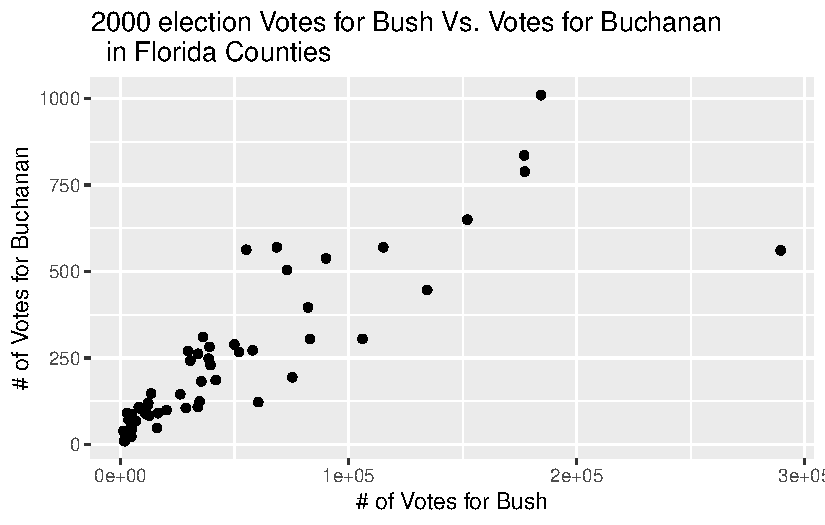
\includegraphics{case-study-template_files/figure-pdf/unnamed-chunk-6-1.pdf}

\begin{Shaded}
\begin{Highlighting}[]
\CommentTok{\# Check conditions for initial model }
\FunctionTok{check\_model}\NormalTok{(election\_model\_bad, }\AttributeTok{check =} \FunctionTok{c}\NormalTok{(}\StringTok{"linearity"}\NormalTok{, }\StringTok{"homogeneity"}\NormalTok{))}
\end{Highlighting}
\end{Shaded}

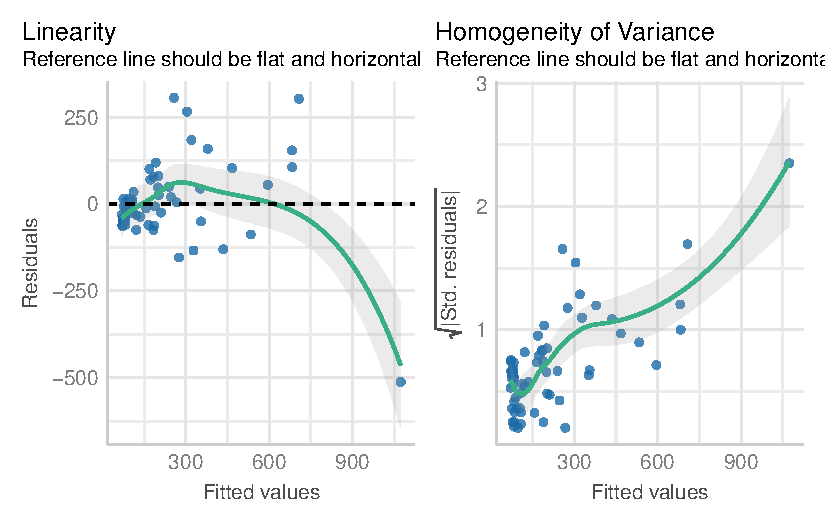
\includegraphics{case-study-template_files/figure-pdf/unnamed-chunk-6-2.pdf}

\begin{Shaded}
\begin{Highlighting}[]
\NormalTok{election\_model\_bad }\SpecialCharTok{|\textgreater{}} \FunctionTok{augment}\NormalTok{() }\SpecialCharTok{|\textgreater{}} \FunctionTok{ggplot}\NormalTok{(}\FunctionTok{aes}\NormalTok{(}\AttributeTok{sample =}\NormalTok{ .resid)) }\SpecialCharTok{+}
  \FunctionTok{geom\_qq}\NormalTok{()}\SpecialCharTok{+} 
  \FunctionTok{geom\_qq\_line}\NormalTok{(}\AttributeTok{col =} \StringTok{"blue"}\NormalTok{)}\SpecialCharTok{+}
  \FunctionTok{labs}\NormalTok{(}\AttributeTok{title =} \StringTok{"Normal Quantile Plot"}\NormalTok{,}
       \AttributeTok{x =} \StringTok{"Theoretical Quantile"}\NormalTok{,}
       \AttributeTok{y =} \StringTok{"Sample Quantile"}\NormalTok{)}
\end{Highlighting}
\end{Shaded}

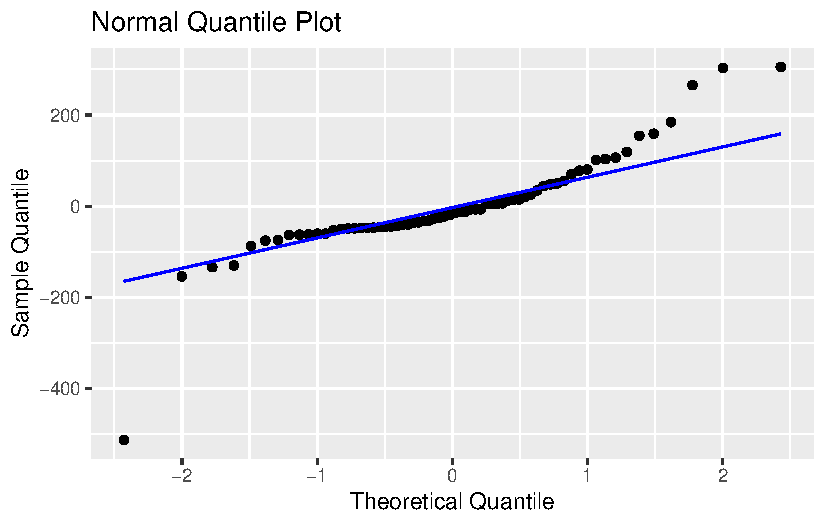
\includegraphics{case-study-template_files/figure-pdf/unnamed-chunk-6-3.pdf}

\begin{Shaded}
\begin{Highlighting}[]
\CommentTok{\# Creating scatter plot sqrt transformed (x)}
\FunctionTok{ggplot}\NormalTok{(}\AttributeTok{data =}\NormalTok{ election\_wo\_pb, }\FunctionTok{aes}\NormalTok{(}\AttributeTok{x =} \FunctionTok{sqrt}\NormalTok{(Bush2000), }\AttributeTok{y =}\NormalTok{ Buchanan2000)) }\SpecialCharTok{+}
  \FunctionTok{geom\_point}\NormalTok{() }\SpecialCharTok{+}
  \FunctionTok{labs}\NormalTok{(}\AttributeTok{x =} \StringTok{"Votes for Bush"}\NormalTok{, }\AttributeTok{y =} \StringTok{"Votes for Buchanan"}\NormalTok{) }\SpecialCharTok{+}
  \FunctionTok{geom\_smooth}\NormalTok{(}\AttributeTok{method =}\NormalTok{ lm, }\AttributeTok{se =} \ConstantTok{FALSE}\NormalTok{)}
\end{Highlighting}
\end{Shaded}

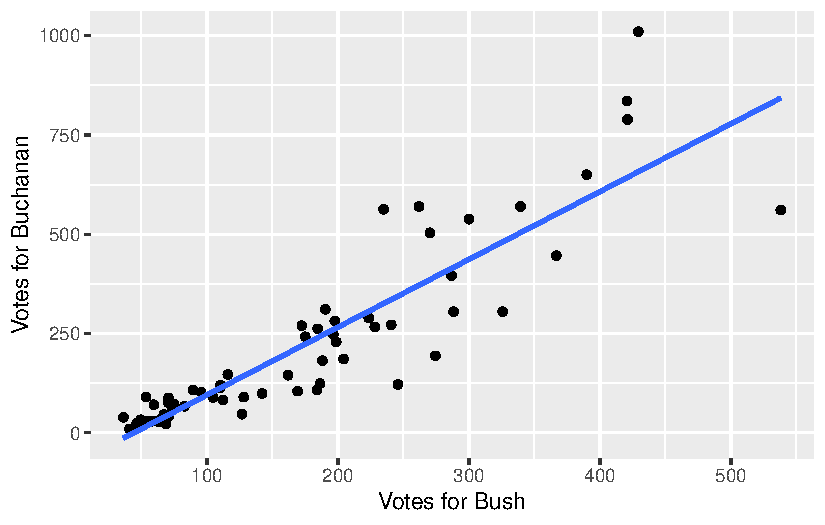
\includegraphics{case-study-template_files/figure-pdf/unnamed-chunk-6-4.pdf}

\begin{Shaded}
\begin{Highlighting}[]
\CommentTok{\# Creating scatter plot sqrt transformed (y)}
\FunctionTok{ggplot}\NormalTok{(}\AttributeTok{data =}\NormalTok{ election\_wo\_pb, }\FunctionTok{aes}\NormalTok{(}\AttributeTok{x =}\NormalTok{ Bush2000, }\AttributeTok{y =} \FunctionTok{sqrt}\NormalTok{(Buchanan2000))) }\SpecialCharTok{+}
  \FunctionTok{geom\_point}\NormalTok{() }\SpecialCharTok{+}
  \FunctionTok{labs}\NormalTok{(}\AttributeTok{x =} \StringTok{"Votes for Bush"}\NormalTok{, }\AttributeTok{y =} \StringTok{"Votes for Buchanan"}\NormalTok{) }\SpecialCharTok{+}
  \FunctionTok{geom\_smooth}\NormalTok{(}\AttributeTok{method =}\NormalTok{ lm, }\AttributeTok{se =} \ConstantTok{FALSE}\NormalTok{)}
\end{Highlighting}
\end{Shaded}

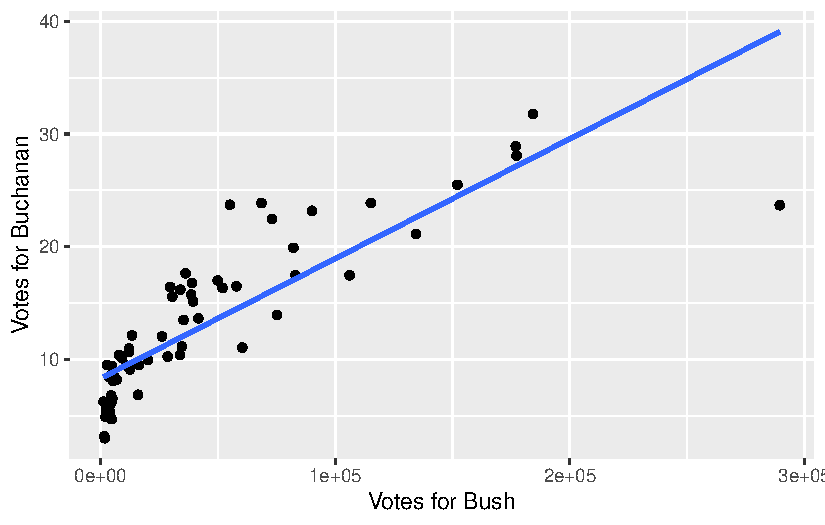
\includegraphics{case-study-template_files/figure-pdf/unnamed-chunk-6-5.pdf}

\begin{Shaded}
\begin{Highlighting}[]
\CommentTok{\# Creating scatter plot sqrt transformed (both)}
\FunctionTok{ggplot}\NormalTok{(}\AttributeTok{data =}\NormalTok{ election\_wo\_pb, }\FunctionTok{aes}\NormalTok{(}\AttributeTok{x =} \FunctionTok{sqrt}\NormalTok{(Bush2000), }\AttributeTok{y =} \FunctionTok{sqrt}\NormalTok{(Buchanan2000))) }\SpecialCharTok{+}
  \FunctionTok{geom\_point}\NormalTok{() }\SpecialCharTok{+}
  \FunctionTok{labs}\NormalTok{(}\AttributeTok{x =} \StringTok{"Votes for Bush"}\NormalTok{, }\AttributeTok{y =} \StringTok{"Votes for Buchanan"}\NormalTok{) }\SpecialCharTok{+}
  \FunctionTok{geom\_smooth}\NormalTok{(}\AttributeTok{method =}\NormalTok{ lm, }\AttributeTok{se =} \ConstantTok{FALSE}\NormalTok{)}
\end{Highlighting}
\end{Shaded}

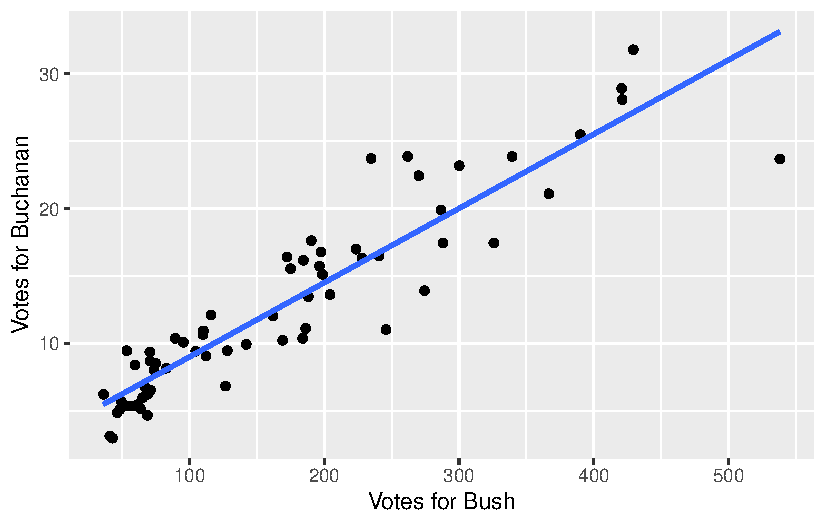
\includegraphics{case-study-template_files/figure-pdf/unnamed-chunk-6-6.pdf}

\begin{Shaded}
\begin{Highlighting}[]
\CommentTok{\# Creating scatter plot log transformed (x)}
\FunctionTok{ggplot}\NormalTok{(}\AttributeTok{data =}\NormalTok{ election\_wo\_pb, }\FunctionTok{aes}\NormalTok{(}\AttributeTok{x =} \FunctionTok{log}\NormalTok{(Bush2000), }\AttributeTok{y =}\NormalTok{ Buchanan2000)) }\SpecialCharTok{+}
  \FunctionTok{geom\_point}\NormalTok{() }\SpecialCharTok{+}
  \FunctionTok{labs}\NormalTok{(}\AttributeTok{x =} \StringTok{"Votes for Bush"}\NormalTok{, }\AttributeTok{y =} \StringTok{"Votes for Buchanan"}\NormalTok{) }\SpecialCharTok{+}
  \FunctionTok{geom\_smooth}\NormalTok{(}\AttributeTok{method =}\NormalTok{ lm, }\AttributeTok{se =} \ConstantTok{FALSE}\NormalTok{)}
\end{Highlighting}
\end{Shaded}

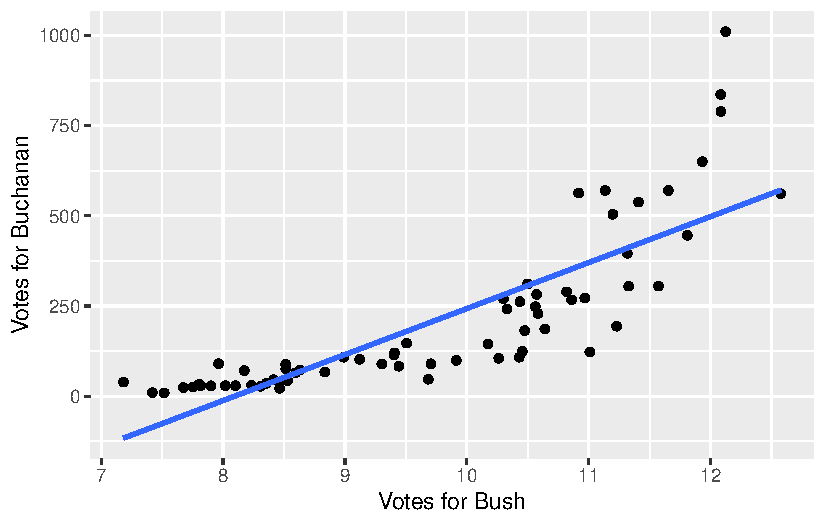
\includegraphics{case-study-template_files/figure-pdf/unnamed-chunk-6-7.pdf}

\begin{Shaded}
\begin{Highlighting}[]
\CommentTok{\# Creating scatter plot log transformed (y)}
\FunctionTok{ggplot}\NormalTok{(}\AttributeTok{data =}\NormalTok{ election\_wo\_pb, }\FunctionTok{aes}\NormalTok{(}\AttributeTok{x =}\NormalTok{ Bush2000, }\AttributeTok{y =} \FunctionTok{log}\NormalTok{(Buchanan2000))) }\SpecialCharTok{+}
  \FunctionTok{geom\_point}\NormalTok{() }\SpecialCharTok{+}
  \FunctionTok{labs}\NormalTok{(}\AttributeTok{x =} \StringTok{"Votes for Bush"}\NormalTok{, }\AttributeTok{y =} \StringTok{"Votes for Buchanan"}\NormalTok{) }\SpecialCharTok{+}
  \FunctionTok{geom\_smooth}\NormalTok{(}\AttributeTok{method =}\NormalTok{ lm, }\AttributeTok{se =} \ConstantTok{FALSE}\NormalTok{)}
\end{Highlighting}
\end{Shaded}

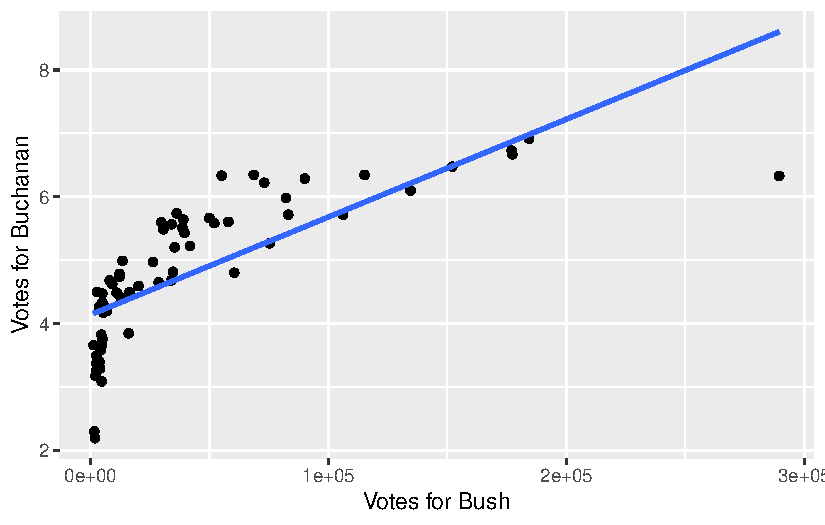
\includegraphics{case-study-template_files/figure-pdf/unnamed-chunk-6-8.pdf}

\begin{Shaded}
\begin{Highlighting}[]
\CommentTok{\# Creating scatter plot log transformed (both) (this one wins!)}
\FunctionTok{ggplot}\NormalTok{(}\AttributeTok{data =}\NormalTok{ election\_wo\_pb, }\FunctionTok{aes}\NormalTok{(}\AttributeTok{x =} \FunctionTok{log}\NormalTok{(Bush2000), }\AttributeTok{y =} \FunctionTok{log}\NormalTok{(Buchanan2000))) }\SpecialCharTok{+}
  \FunctionTok{geom\_point}\NormalTok{() }\SpecialCharTok{+}
  \FunctionTok{labs}\NormalTok{(}\AttributeTok{x =} \StringTok{"Votes for Bush"}\NormalTok{, }\AttributeTok{y =} \StringTok{"Votes for Buchanan"}\NormalTok{) }\SpecialCharTok{+}
  \FunctionTok{geom\_smooth}\NormalTok{(}\AttributeTok{method =}\NormalTok{ lm, }\AttributeTok{se =} \ConstantTok{FALSE}\NormalTok{)}
\end{Highlighting}
\end{Shaded}

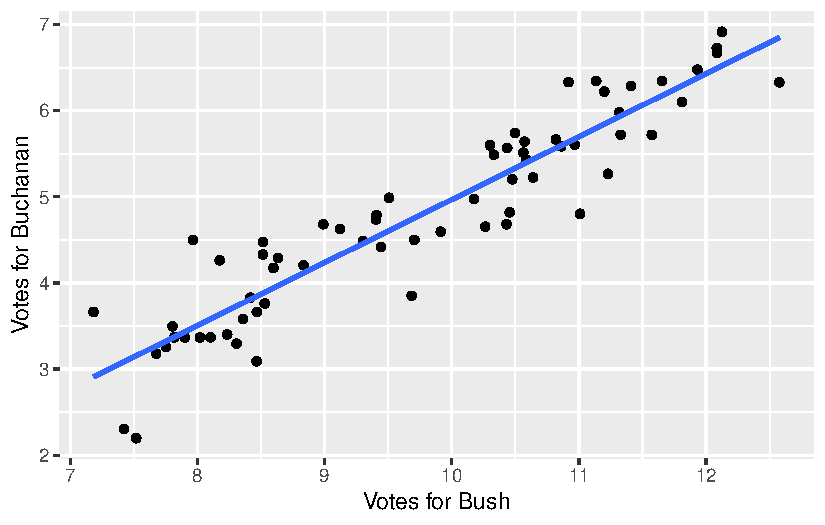
\includegraphics{case-study-template_files/figure-pdf/unnamed-chunk-6-9.pdf}

\begin{Shaded}
\begin{Highlighting}[]
\CommentTok{\# Log Transformed Model}
\NormalTok{election\_model }\OtherTok{\textless{}{-}} \FunctionTok{lm}\NormalTok{(}\FunctionTok{log}\NormalTok{(Buchanan2000) }\SpecialCharTok{\textasciitilde{}} \FunctionTok{log}\NormalTok{(Bush2000), }\AttributeTok{data =}\NormalTok{ election\_wo\_pb)}
\FunctionTok{summary}\NormalTok{(election\_model)}
\end{Highlighting}
\end{Shaded}

\begin{verbatim}

Call:
lm(formula = log(Buchanan2000) ~ log(Bush2000), data = election_wo_pb)

Residuals:
     Min       1Q   Median       3Q      Max 
-0.95631 -0.21236  0.02503  0.28102  1.02056 

Coefficients:
              Estimate Std. Error t value Pr(>|t|)    
(Intercept)   -2.34149    0.35442  -6.607 9.07e-09 ***
log(Bush2000)  0.73096    0.03597  20.323  < 2e-16 ***
---
Signif. codes:  0 '***' 0.001 '**' 0.01 '*' 0.05 '.' 0.1 ' ' 1

Residual standard error: 0.4198 on 64 degrees of freedom
Multiple R-squared:  0.8658,    Adjusted R-squared:  0.8637 
F-statistic:   413 on 1 and 64 DF,  p-value: < 2.2e-16
\end{verbatim}

\begin{Shaded}
\begin{Highlighting}[]
\CommentTok{\# Checking conditions for transformed model }
\FunctionTok{check\_model}\NormalTok{(election\_model, }\AttributeTok{check =} \FunctionTok{c}\NormalTok{(}\StringTok{"linearity"}\NormalTok{, }\StringTok{"homogeneity"}\NormalTok{))}
\end{Highlighting}
\end{Shaded}

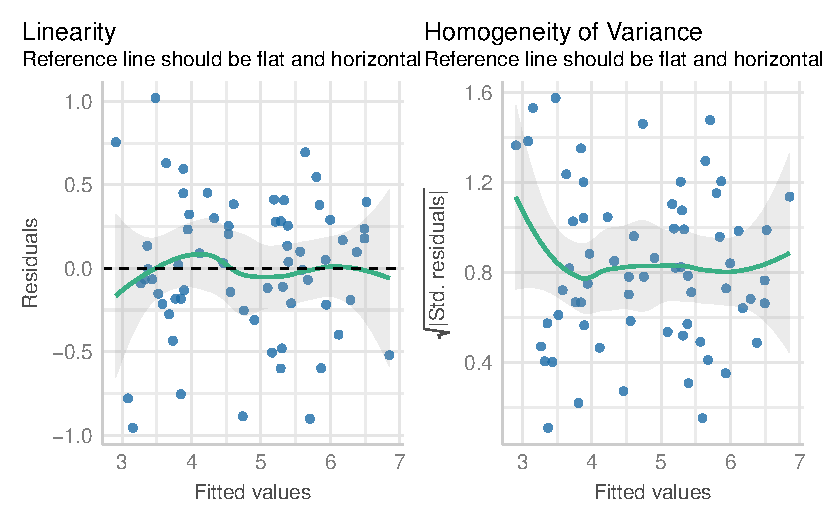
\includegraphics{case-study-template_files/figure-pdf/unnamed-chunk-6-10.pdf}

\begin{Shaded}
\begin{Highlighting}[]
\NormalTok{election\_model }\SpecialCharTok{|\textgreater{}} \FunctionTok{augment}\NormalTok{() }\SpecialCharTok{|\textgreater{}} \FunctionTok{ggplot}\NormalTok{(}\FunctionTok{aes}\NormalTok{(}\AttributeTok{sample =}\NormalTok{ .resid)) }\SpecialCharTok{+}
  \FunctionTok{geom\_qq}\NormalTok{()}\SpecialCharTok{+} 
  \FunctionTok{geom\_qq\_line}\NormalTok{(}\AttributeTok{col =} \StringTok{"blue"}\NormalTok{)}\SpecialCharTok{+}
  \FunctionTok{labs}\NormalTok{(}\AttributeTok{title =} \StringTok{"Normal Quantile Plot"}\NormalTok{,}
       \AttributeTok{x =} \StringTok{"Theoretical Quantile"}\NormalTok{,}
       \AttributeTok{y =} \StringTok{"Sample Quantile"}\NormalTok{)}
\end{Highlighting}
\end{Shaded}

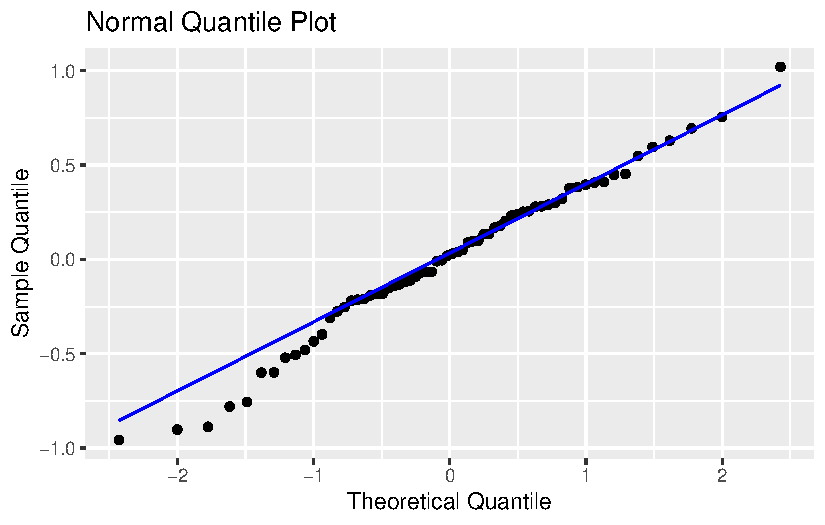
\includegraphics{case-study-template_files/figure-pdf/unnamed-chunk-6-11.pdf}

\begin{Shaded}
\begin{Highlighting}[]
\CommentTok{\# Making prediction interval}
\NormalTok{palm\_beach }\OtherTok{\textless{}{-}} \FunctionTok{data.frame}\NormalTok{(}\AttributeTok{Bush2000 =} \FunctionTok{c}\NormalTok{(}\DecValTok{152846}\NormalTok{))}
\FunctionTok{augment}\NormalTok{(election\_model, }\AttributeTok{newdata =}\NormalTok{ palm\_beach, }\AttributeTok{interval =} \StringTok{"prediction"}\NormalTok{)}
\end{Highlighting}
\end{Shaded}

\begin{verbatim}
# A tibble: 1 x 4
  Bush2000 .fitted .lower .upper
     <dbl>   <dbl>  <dbl>  <dbl>
1   152846    6.38   5.52   7.24
\end{verbatim}

\begin{Shaded}
\begin{Highlighting}[]
\NormalTok{lower }\OtherTok{\textless{}{-}} \FunctionTok{exp}\NormalTok{(}\FloatTok{5.52}\NormalTok{)}
\NormalTok{fitted }\OtherTok{\textless{}{-}} \FunctionTok{exp}\NormalTok{(}\FloatTok{6.38}\NormalTok{)}
\NormalTok{upper }\OtherTok{\textless{}{-}} \FunctionTok{exp}\NormalTok{(}\FloatTok{7.24}\NormalTok{)}

\NormalTok{equation }\OtherTok{\textless{}{-}} \FunctionTok{extract\_eq}\NormalTok{(election\_model, }\AttributeTok{use\_coefs =} \ConstantTok{TRUE}\NormalTok{)}

\CommentTok{\# Extract coefficients from model }
\NormalTok{votes\_table }\OtherTok{\textless{}{-}} \FunctionTok{summary}\NormalTok{(election\_model)}\SpecialCharTok{$}\NormalTok{coefficients}

\CommentTok{\# Display coefficients in (pretty) table }
\NormalTok{votes\_table }\SpecialCharTok{|\textgreater{}} \FunctionTok{kbl}\NormalTok{(}\AttributeTok{col.names =} \FunctionTok{c}\NormalTok{(}\StringTok{"Estimate"}\NormalTok{, }\StringTok{"Std. Error"}\NormalTok{, }\StringTok{"t value"}\NormalTok{, }\StringTok{"P{-}value"}\NormalTok{), }\AttributeTok{align =} \StringTok{"c"}\NormalTok{, }\AttributeTok{booktabs =}\NormalTok{ T, }\AttributeTok{linesep=}\StringTok{""}\NormalTok{, }\AttributeTok{digits =} \FunctionTok{c}\NormalTok{(}\DecValTok{2}\NormalTok{, }\DecValTok{2}\NormalTok{, }\DecValTok{2}\NormalTok{, }\DecValTok{4}\NormalTok{)) }\SpecialCharTok{|\textgreater{}} \FunctionTok{kable\_classic}\NormalTok{(}\AttributeTok{full\_width =}\NormalTok{ F, }\AttributeTok{latex\_options =} \FunctionTok{c}\NormalTok{(}\StringTok{"HOLD\_position"}\NormalTok{))}
\end{Highlighting}
\end{Shaded}

\begin{table}[H]
\centering
\begin{tabular}[t]{lcccc}
\toprule
  & Estimate & Std. Error & t value & P-value\\
\midrule
(Intercept) & -2.34 & 0.35 & -6.61 & 0\\
log(Bush2000) & 0.73 & 0.04 & 20.32 & 0\\
\bottomrule
\end{tabular}
\end{table}



\end{document}
